\chapter{Alimentation d’un microprocesseur}

On souhaite alimenter un microprocesseur STM32H4 à l'aide d'une batterie. Le cahier des charges est le suivant :

\begin{itemize}
\item Batterie LiPo 2S $V_{in} = 7.4\ V$
\item Tension d’alimentation du microprocesseur : $V_{out}=3.3\ V$
\item Ondulation de tension max en entrée du microprocesseur : $\Delta V_S = 50\ mV$
\item Courant nominal de sortie : $I_S = 200\ mA$
\item Ondulation de courant : 30\%
\end{itemize}

Pour cela, on souhaite utiliser le composant suivant : \textbf{LT1959} dont un extrait de la documentation est en annexe. On supposera dans cet exercice que les \underline{\textbf{composants sont}} \underline{\textbf{parfaits}}, et que le Buck fonctionne en régime de \underline{\textbf{conduction continue}}.

\begin{enumerate}

\item \textbf{Étude du Buck}

\begin{enumerate}

\item Tracer le circuit permettant d'utiliser ce composant en fonctionnement Buck (la valeur des composants passifs n'est pas demandée). Pour la broche 6 $\overline{SHDN}$, on supposera que le Buck est toujours en fonctionnement.

\begin{center}
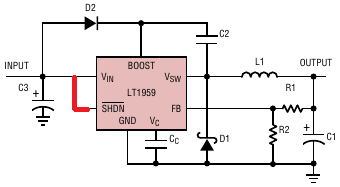
\includegraphics[width=0.8\linewidth]{TD_Buck/Correction/fig/Q1_1.png}
\end{center}

\item On suppose que le processeur absorbe un courant $I_s$ constant égal au courant nominal et que la tension de sortie est constante (on néglige l'ondulation de la tension de sortie). Tracer l'allure de la tension $V_{SW}$ en sortie du composant \textbf{LT1959}, la tension $V_{ce}$ aux bornes du transistor $Q_1$ et le courant $I_{L}$ dans l'inductance de sortie. En déduire la relation entre la tension d'entrée $V_{in}$, $V_{out}$ et le rapport cyclique $\alpha$ du hacheur.

\begin{center}
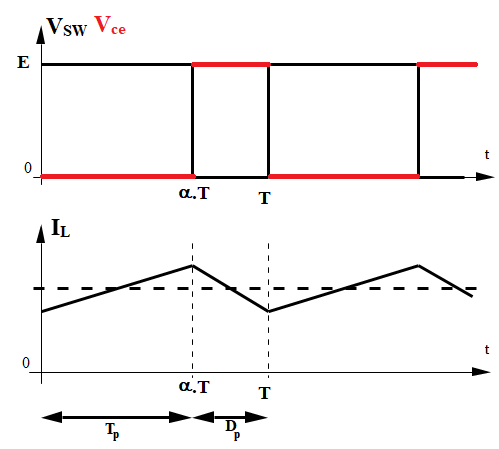
\includegraphics[width=0.7\linewidth]{TD_Buck/Correction/fig/Q1_2.png}

$V_{out}=<V_{SW}>=\alpha V_{in}$
\end{center}

\item Si la tension de sortie est bien régulée, quelle sera la valeur du rapport cyclique $\alpha_n$ imposé par le \textbf{LT1959} ?

\begin{center}
$\alpha=\dfrac{V_{out}}{V_{in}}=\dfrac{3.3}{7.4}\approx0.45$
\end{center}

\item Justifier que ce composant est adapté au cahier des charges. Peut-on utiliser une batterie LiPo 1S ($3.7 V$) à la place de la LiPo 2S ?

\begin{center}
Tension d'entrée min : 4 V $\rightarrow V_{in}>4\ V$

Tension de sortie min : 1.21 V $\rightarrow V_{out}>1.21\ V$

Courant de commutation max : 4.5 A $\rightarrow$ Courant à commuter : $I_S+\Delta I_s/2 =0.2+0.2*0.15=0.23<4.5\ A$

LiPo 1S : $3.7\ V < 4\ V\ \rightarrow$ ne peut pas fonctionner directement avec ce composant
\end{center}

\item A partir de la documentation, quelle est la fréquence de découpage du hacheur ?

\begin{center}
$f_{SW}=500\ kHz$
\end{center}

\item Calculer l'ondulation de courant $\Delta I_{L}$ dans l'inductance de sortie, en fonction de l'inductance $L_1$ placée. En déduire la valeur de l'inductance afin de respecter le cahier des charges.

\begin{center}
Entre 0 et $\alpha T$ : $V_L=V_{in}-V_{out}=L\dfrac{dI_L}{dt} \rightarrow \Delta I_L=(V_{in}-V{out}).\dfrac{\alpha T}{L}$

$\Delta I_L=\dfrac{\alpha .(1-\alpha).V_{in}.T}{L}$

$L>61\mu H$
\end{center}

\item Tracer la tension de sortie en tenant compte de l'ondulation de tension. Calculer la valeur du condensateur de sortie $C_1$ à choisir afin de respecter le cahier des charges.

\begin{center}
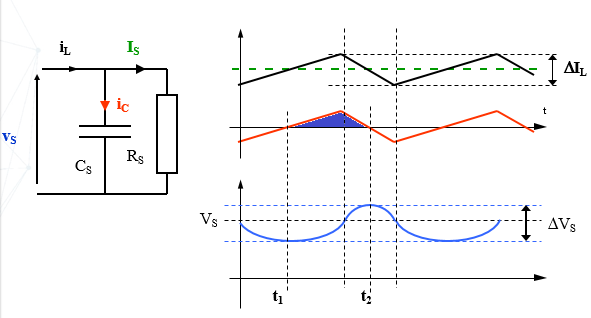
\includegraphics[width=0.7\linewidth]{TD_Buck/Correction/fig/Q1_7.png}

$$t_1=\dfrac{\alpha.T}{2}\ \ \ \ \  t_2=\dfrac{(1+\alpha).T}{2}$$

$$\Delta V_C=\dfrac{1}{C_1}\int_{t_1}^{t_2}i_C(t).dt=\dfrac{1}{C_1}.\dfrac{1}{2}.\dfrac{\Delta I_S}{2}.(t_2-t_1)$$

$$\rightarrow C_S=\dfrac{\alpha.(1-\alpha).V_{in}}{8.f_{SW}^2.L.\Delta V_S}=300\ nF$$
\end{center}

\item Que se passe-t-il si le microprocesseur consomme peu de courant (mode veille par exemple) ?

\begin{center}
Conduction discontinue $\rightarrow$ si $\alpha$ est fixe, $V_S$ augmente (potentiellement jusqu'à $V_{in}=7.4\ V$ si le processeur ne consomme aucun courant)
\end{center}

\end{enumerate}

\item \textbf{Etude de la commande}

Dans cette partie, on s'intéresse à la commande du Buck. Pour cela, on utilise le schéma simplifié suivant :

\begin{figure}[h]
\centering
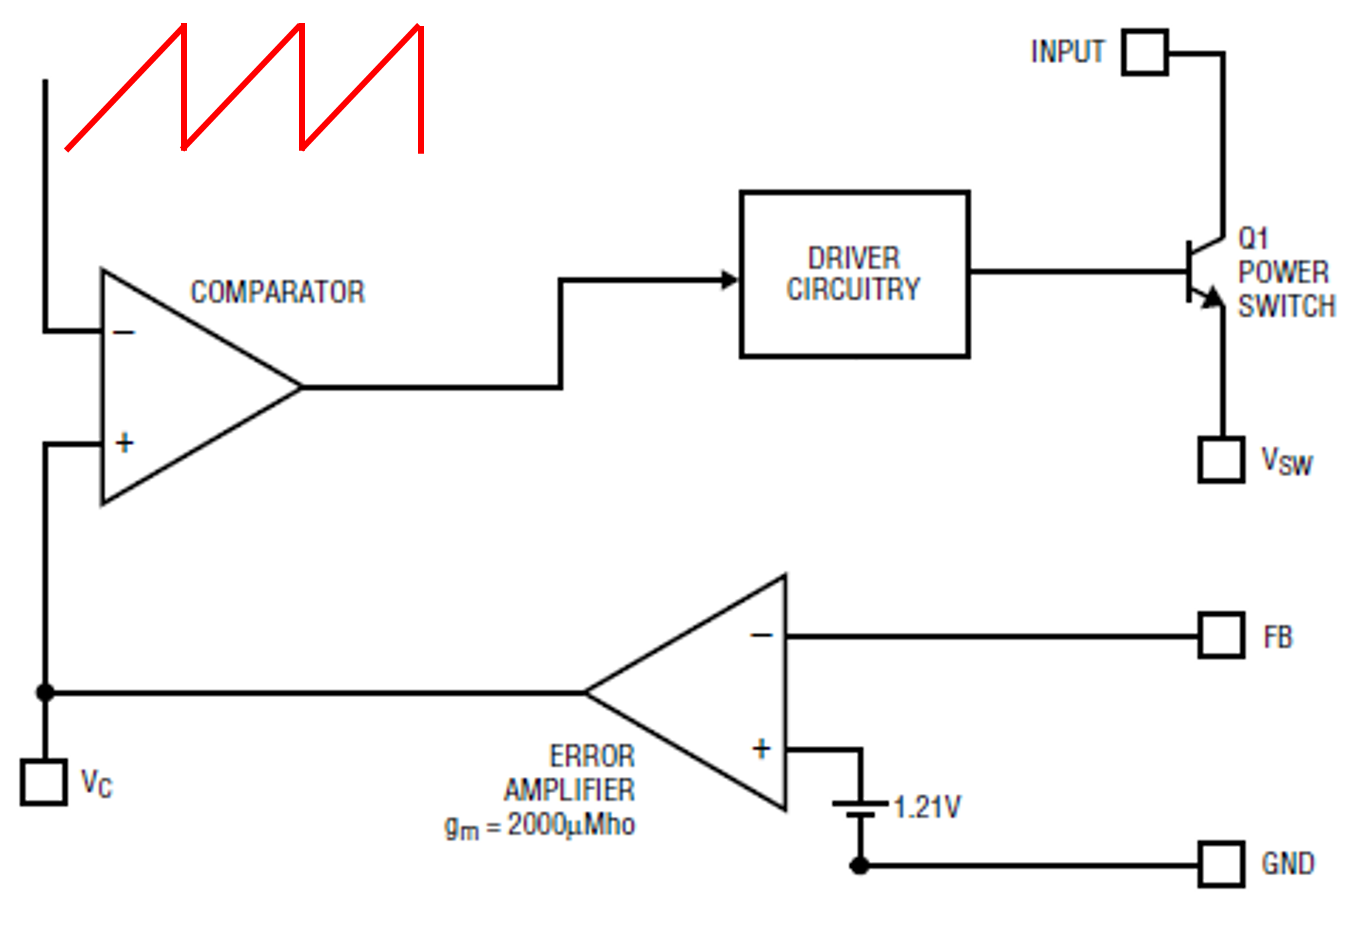
\includegraphics[width=0.8\linewidth]{TD_Buck/fig/Buck_regul.png}
\caption{Simplified internal control}
\end{figure}

Le signal en dent de scie évolue entre 0 et 2 V, avec une fréquence égale à la fréquence de découpage du hacheur. 

\begin{enumerate}

\item Choisir les valeurs des résistances à connecter sur la broche \textit{FB} afin d'avoir la tension de sortie demandée. On utilisera pour cela les valeurs de résistances de la série E12.

(Valeurs de la série E12 : 100, 120, 150, 180, 220, 270, 330, 390, 470, 560, 680, 820).

\begin{center}
Pont diviseur de tension : $\dfrac{R_2}{R_1+R_2}=\dfrac{1.21}{3.3}\rightarrow R_1\approx 1.73.R_2$
$$R_1=470\ k\Omega\ \ \ \ \ \ \ R_2=270\ k\Omega$$
\end{center}


\item Pour une tension $V^+=0.5 V$ à l'entrée du comparateur, tracer le signal en sortie du comparateur. En déduire l'expression qui lie la tension $V^+$ du comparateur et la valeur du rapport cyclique $\alpha$ du hacheur.

\begin{center}
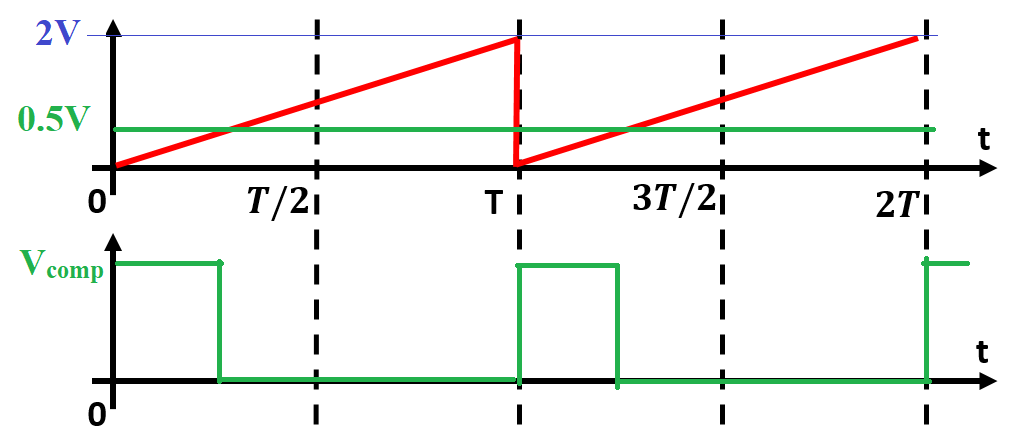
\includegraphics[width=0.7\linewidth]{TD_Buck/Correction/fig/Q2_1.png}
$$V^+=2.\alpha$$

\end{center}

On modélise le convertisseur asservi avec le schéma bloc suivant :

\begin{figure}[H]
\centering
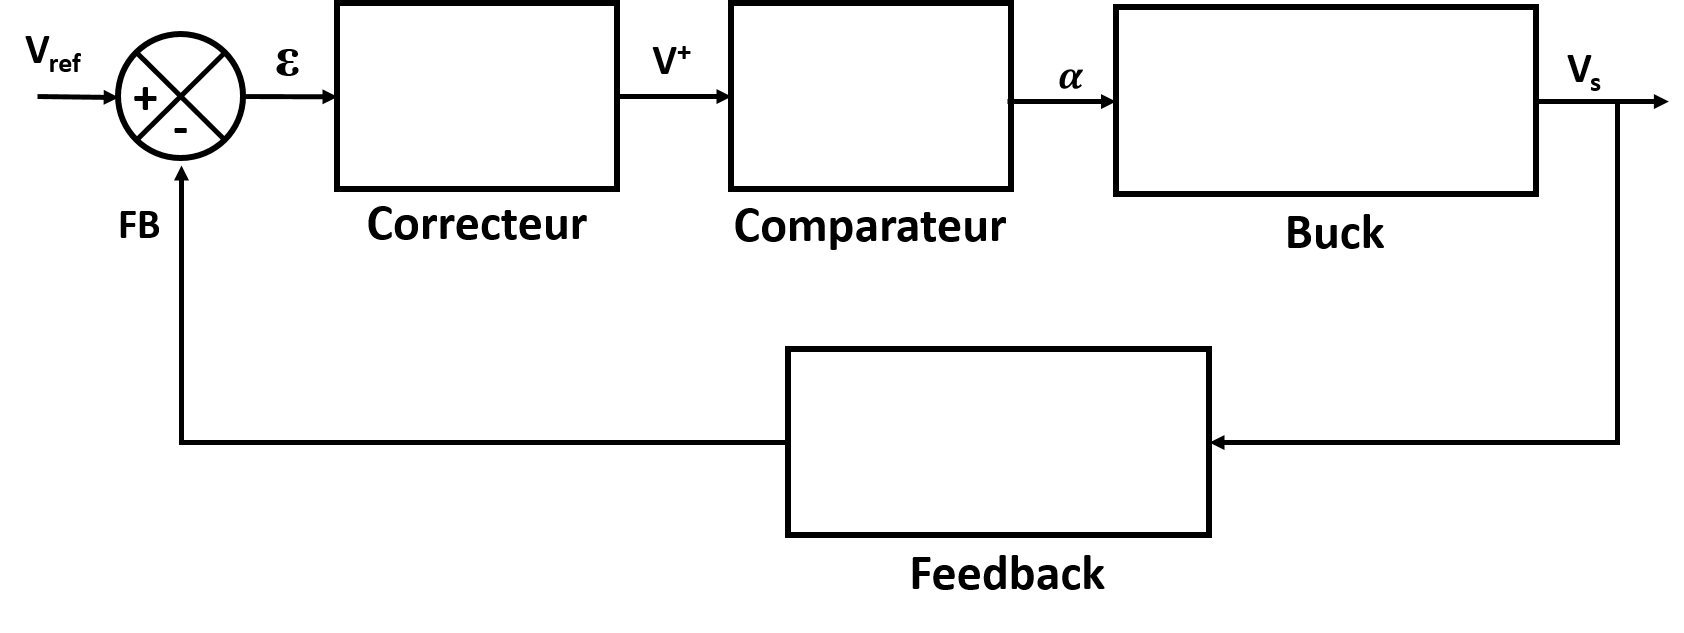
\includegraphics[width=0.8\linewidth]{TD_Buck/fig/Buck_regul_1.png}
\caption{Global bloc diagramm}
\end{figure}

\item Compléter le bloc ``\textit{Comparateur}''. A l'aide de la partie 1, compléter le bloc ``\textit{Feedback}''

Le bloc ``\textit{Buck}'' est modélisé par un gain statique $K$ correspondant à $\dfrac{V_{s\ moy}}{\alpha}$ et une fonction de transfert correspondant au filtre de sortie de Buck. La résistance $R_m$ symbolise l'impédance d'entrée du microcontrôleur.

\begin{figure}[h]
\centering
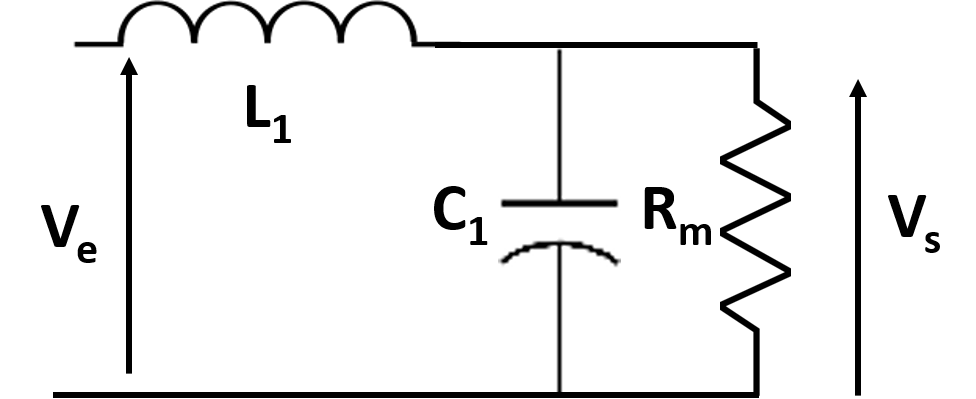
\includegraphics[width=0.65\linewidth]{TD_Buck/fig/Buck_filtre.png}
\caption{Equivalent schematic of the Buck}
\end{figure}

\item Rappeler les valeurs de $L$ et $C$ déterminées à la partie. Déterminer la valeur de $R_m$ lorsque le microcontrôleur absorbe le courant nominal.

\begin{center}

$L=61\ \mu H\ \ \ \ \ \ C=300\ nF$

$R_m=\dfrac{V_{out}}{I_S}=16.5\ \Omega$
\end{center}

\item Déterminer la fonction de transfert correspondant au bloc ``\textit{Buck}''.

\begin{center}
$\dfrac{V_s}{V_e}=\dfrac{1}{1+j.\frac{L_1}{R_m}.\omega-L_1.C_1.\omega^2}$

Fonction de transfert du Buck : $\dfrac{V_s}{\alpha}=\dfrac{V_{in}}{1+j.\frac{L_1}{R_m}.\omega-L_1.C_1.\omega^2}$
\end{center}

\item On place sur la broche $V_c$ un circuit $RC$ série. On suppose que le courant en entrée du comparateur est nul (haute impédance d'entrée). Le bloc ``\textit{Correcteur}'' est donc un proportionnel intégral de la forme $C(p) = K_p(1+\dfrac{1}{T_i.p})$. Déterminer les valeurs de $K_p$ et $T_i$ en fonction de $R$, $C$ et $g_m$.

\begin{center}
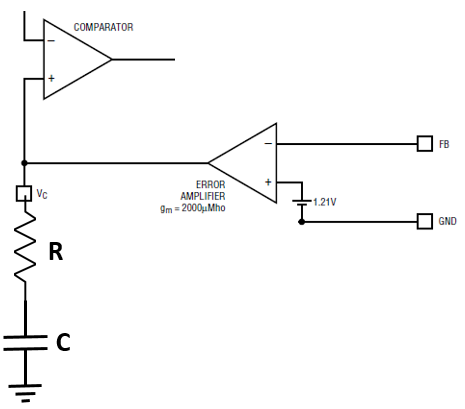
\includegraphics[width=0.55\linewidth]{TD_Buck/Correction/fig/Q2_6.png}
$V^+(j\omega)=(R+\dfrac{1}{j.C.\omega}).I(j\omega)=(R+\dfrac{1}{j.C.\omega}).g_m.\epsilon(j\omega)$

$\dfrac{V^+}{\epsilon}=(R+\dfrac{1}{j.C.\omega}).g_m=R.g_m.(1+\frac{1}{j.R.C.\omega})$

$K_p=R.g_m\ \ \ \ \ \ \ \ \ \ \ \ T_i=R.C$
\end{center}

\item Calculer $R$ afin que le rapport cyclique au démarrage soit environ égal à $\dfrac{\alpha_n}{2}$ et $C$ pour avoir une constante de temps du correcteur 10 fois supérieure à la constante de temps du système non corrigé.

\begin{center}
Au démarrage : $V_{FB}=0$ et le condensateur est déchargé : $V^+=R.g_m.\epsilon=1.2R.g_m$

$\alpha=0.5*1.2R.g_m\rightarrow R=\dfrac{\alpha}{0.6g_m}=186\Omega$

Constante de temps du correcteur : $T_i=R.C>10\sqrt{L_1.C_1}\rightarrow C>\dfrac{10}{R}.\sqrt{L_1.C_1}=230\ nF$
\end{center}

\item En régime établi, déterminer le courant de sortie de l'ampli d'erreur et les tensions aux bornes de $R$, $C$ et $V_c$. En déduire le rapport cyclique et comparer au résultat du 1.3.

Quand t$->$ $\infty$, $\epsilon -> 0$ (thérome de la valeure finale) donc le courant de sortie de l'ampli est nul. 

On a donc $V_{FB}=1.21\ V$ soit $V_{out}=3.3\ V$ comme désiré.

De même, théorme de la valeure finale, $\alpha$ tend vers $\dfrac{R_1+R_2}{R_2}.\dfrac{V_{ref}}{V_{in}}=0.44$


\end{enumerate}

\end{enumerate}

\newpage
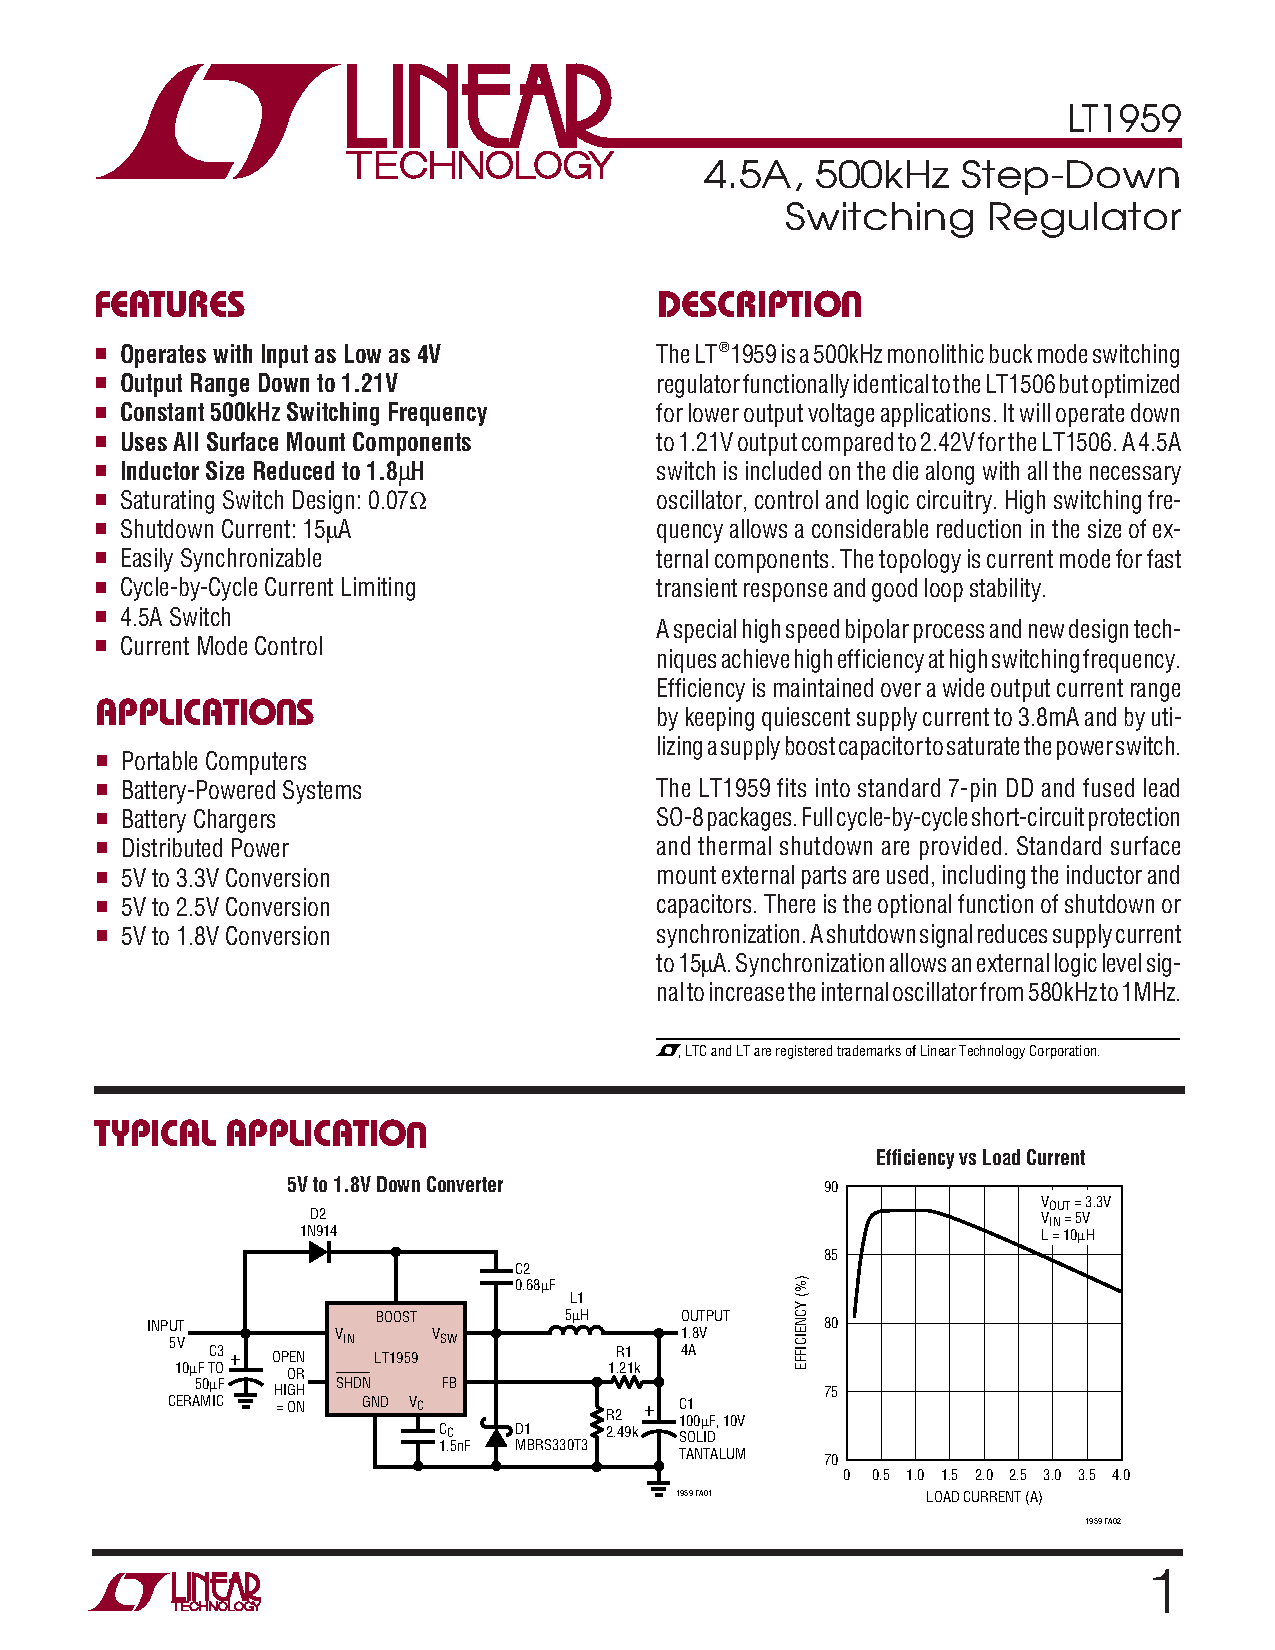
\includepdf[pages=1-4]{TD_Buck/fig/LT1959.pdf}
\includepdf[pages=6-7]{TD_Buck/fig/LT1959.pdf}